\documentclass[12pt,a4paper]{article}
%\usepackage{ctex}
\usepackage{amsmath,amscd,amsbsy,amssymb,latexsym,url,bm,amsthm}
\usepackage{epsfig,graphicx,subfigure}
\usepackage{enumitem,balance}
\usepackage{wrapfig}
\usepackage{mathrsfs,euscript}
\usepackage[x11names,svgnames,dvipsnames]{xcolor}
\usepackage{hyperref}
\usepackage[vlined,ruled,commentsnumbered,linesnumbered]{algorithm2e}
\usepackage{listings}
\usepackage{multicol}
%\usepackage{fontspec}

\renewcommand{\listalgorithmcfname}{List of Algorithms}
\renewcommand{\algorithmcfname}{Alg.}
\newtheorem{theorem}{Theorem}
\newtheorem{lemma}[theorem]{Lemma}
\newtheorem{proposition}[theorem]{Proposition}
\newtheorem{corollary}[theorem]{Corollary}
\newtheorem{exercise}{Exercise}
\newtheorem*{solution}{Solution}
\newtheorem{definition}{Definition}
\theoremstyle{definition}


%\numberwithin{equation}{section}
%\numberwithin{figure}{section}

\renewcommand{\thefootnote}{\fnsymbol{footnote}}

\newcommand{\postscript}[2]
 {\setlength{\epsfxsize}{#2\hsize}
  \centerline{\epsfbox{#1}}}

\renewcommand{\baselinestretch}{1.0}

\setlength{\oddsidemargin}{-0.365in}
\setlength{\evensidemargin}{-0.365in}
\setlength{\topmargin}{-0.3in}
\setlength{\headheight}{0in}
\setlength{\headsep}{0in}
\setlength{\textheight}{10.1in}
\setlength{\textwidth}{7in}
\makeatletter \renewenvironment{proof}[1][Proof] {\par\pushQED{\qed}\normalfont\topsep6\p@\@plus6\p@\relax\trivlist\item[\hskip\labelsep\bfseries#1\@addpunct{.}]\ignorespaces}{\popQED\endtrivlist\@endpefalse} \makeatother
\makeatletter
\renewenvironment{solution}[1][Solution] {\par\pushQED{\qed}\normalfont\topsep6\p@\@plus6\p@\relax\trivlist\item[\hskip\labelsep\bfseries#1\@addpunct{.}]\ignorespaces}{\popQED\endtrivlist\@endpefalse} \makeatother


\definecolor{codegreen}{rgb}{0.44,0.68,0.28}
\definecolor{codegray}{rgb}{0.5,0.5,0.5}
\definecolor{codepurple}{rgb}{0.58,0,0.82}
\definecolor{backcolour}{rgb}{0.96,0.96,0.96}

\lstset{
language=C++,
frame=shadowbox,
keywordstyle = \color{blue}\bfseries,
commentstyle=\color{codegreen},
tabsize = 4,
backgroundcolor=\color{backcolour},
numbers=left,
numbersep=5pt,
breaklines=true,
emph = {int,float,double,char},emphstyle=\color{orange},
emph ={[2]const, typedef},emphstyle = {[2]\color{red}} }



\begin{document}
\noindent

%========================================================================
\noindent\framebox[\linewidth]{\shortstack[c]{
\Large{\textbf{Lab08-Graphs}}\vspace{1mm}\\
VE281 - Data Structures and Algorithms, Xiaofeng Gao, TA: Li Ma, Autumn 2019}}
%CS26019 - Algorithm Design and Analysis, Xiaofeng Gao, Autumn 2019}}
\begin{center}
\footnotesize{\color{red}$*$ Please upload your assignment to website. Contact webmaster for any questions.}

\footnotesize{\color{blue}$*$ Name:Jintian Ge  \quad Student ID:517021911142 \quad Email: gejintian@sjtu.edu.cn}
\end{center}


\begin{enumerate}

\item \textbf{DAG.} Suppose that you are given a directed acyclic graph $G=(V,E)$ with real-valued edge weights and two distinct nodes $s$ and $d$. Describe an algorithm for finding a longest weighted simple path from $s$ to $d$. For example, for the graph shown in Figure 1, the longest path from node $A$ to node $C$ should be $A \rightarrow B \rightarrow F \rightarrow C$. If there is no path exists between the two nodes, your algorithm just tells so. What is the efficiency of your algorithm? (Hint: consider topological sorting on the DAG.)

\begin{solution}
Basic idea is that firstly we use topological sorting to realize linearization. Then, we cut off the interval between s and d. Here we get $[s,v_0,v_1,v_2,...,d]$. Next, we go through these vertex and delete all vertexes which cannot be inversely reached by u. Then, we use a vector $DQ$ to contain these nodes. For each node, it has: a string presenting its name, and an indicator. An indicator is a pair, in which one is a pointer to another node and one is the total cost that the corresponding node will bring. We will make sure that $indicate.cost$ is the largest. When we reach s, we will visit the indicator, and go through the path. Finally we will find the longest path. If s has no indicator, then there is no path from s to d.

In this graph, for example, if we want path from A to C, then node B in the vector $DQ$ has two members: a sting 'B', which is its name, and an indicator that containing a pair: \{Pointer to F(\&F), cost: 11\}. In the tracing back part, when we visit B we will choose F as the next node to visit.

For efficiency, there are two parts of this algorithm might affect the efficiency. In the topological sort and delete part, it needs $O(|E|)$ work at most.
 In find path part, in the worst case(all vertexes are included) we need $O(|V|)$ work.
 Therefore the overall time complexity should be $O(|V|+|E|)$.
 
 The following is the two structures I mentioned before and the pseudo code of the algorithm.
 
\begin{lstlisting}[language=C++]
struct indicator{
	node *pointer;
	int cost;
};
struct node{
	string name;
	indicator indicate;
};
\end{lstlisting}
\begin{minipage}[t]{0.9\textwidth}
\begin{algorithm}[H]
	\BlankLine
	\SetKwInOut{Input}{input}
	\SetKwInOut{Output}{output}
	\caption{LongestPathSelect}\label{Alg_LongestPathSelect}
	\Input{A directed acyclic graph G=(V,E), two distinct vertices s and d.}
	\Output{Longest path from s to d}
	\BlankLine
    L=TopologicalSorting(G)\;
    Cut off L such that M starts from s and ends at d\;
    EXPLORE(d) with all path inverse\;
    Delete vertices in M which were not be reached in EXPLORE(d) with all path inverse\;
    vector<node> DQ\;
    \For{$n$ \textbf{in} $L$}{
        node $n(None, 0)$\;
        DQ.PushBack(n)\;
    }
    \While{\textbf{not} DQ.empty()}{
        $v \leftarrow DQ.PopBack()$\;
        \If{$(ForwardEdge(u,v)\in V) \&\& (u\in L)$}{
            \If{$u.indicate.cost < v.indicate.cost + PathWeight(u,v)$}{
                $u.indicate.cost \leftarrow v.indicate.cost + PathWeight(u,v)$\;
                $u.indicate.pointer\leftarrow \&v$\;
            }
        }
    }
    $vector<string> Path$\;
    \If{s.vect.empty()}{
        \Return{\textbf{No path}}\;
    }
    \Else{
        $v \leftarrow s$\;
        \While{\textbf{not} $v.vect.empty()$}{
            $p\leftarrow *v.indicate.pointer$\;
            $Path$.pushBack(p.name)\;
            $v \leftarrow p$\;
        }
        \Return{$Path$}\;
    }
\end{algorithm}
\end{minipage}
\end{solution}

\begin{figure}[htbp]
% \begin{minipage}[t]{0.5\linewidth}
% \centering
% 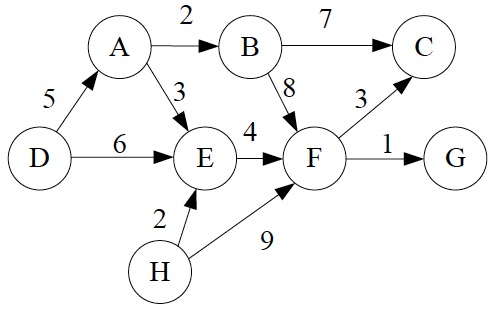
\includegraphics[scale=0.35]{Lab08-figure1.jpg}
% \caption{A weighted undirected graph.}
% \end{minipage}%
% \begin{minipage}[t]{0.5\linewidth}
\centering
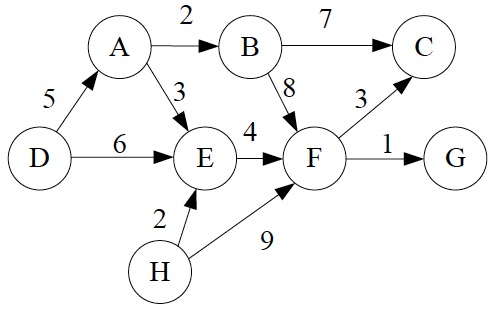
\includegraphics[scale=0.35]{Lab08-figure1.jpg}
\caption{A weighted directed graph.}
% \end{minipage}
\end{figure}

\item \textbf{ShortestPath.} Suppose that you are given a directed graph $G=(V,E)$ on which each edge $(u,v) \in E$ has an associated value $r(u,v)$, which is a real number in the range $0 \leq r(u,v) \leq 1$ that represents the reliability of a communication channel from vertex $u$ to vertex $v$. We interpret $r(u,v)$ as the probability that the channel from $u$ to $v$ will not fail, and we assume that these probabilities are independent. Give an efficient algorithm to find the most reliable path between two given vertices.

\begin{solution}
Basic idea is using Dijkstra's Algorithm. Meanwhile, each time we calculate reliability, we use multiply instead of add. And we update the value of each vertex if and only if $r(s,u)>r[u]$. Also, we will store the predecessor which causing the maximum reliability in that vertex.

\begin{minipage}[t]{0.9\textwidth}
\begin{algorithm}[H]
	\BlankLine
	\SetKwInOut{Input}{input}
	\SetKwInOut{Output}{output}
	\caption{ReliablePathSelect}\label{Alg_ReliablePathSelect}
	\Input{A directed graph G=(V,E), two distinct vertices s and d.}
	\Output{Most reliable path from s to d}
	\BlankLine
	$s.r\leftarrow 0$\;
	$s.predecessor \leftarrow None$\;
	INSERT(Q,s)\;
    \ForEach{$u \in V/{s}$}{
        $u.r \leftarrow 0$
        INSERT(Q,u)\;
    }
    
    \While{$Q \neq \emptyset$}{
        $u\leftarrow EXTRACT-MAX(Q)$\;
        $S\leftarrow S\cup \{u\}$\;
        \ForEach{v \in Adj[u]}{
            \If{$v.r<u.r\times r(u,v)$}{
                $v.r\leftarrow u.r\times r(u,v)$\;
                $v.predecessor\leftarrow u$\;
                DECREASE-KEY(Q,v)\;
            }
        }
    }
    \Return{$TraceBack(s,d)$}\;
\end{algorithm}
\end{minipage}

\end{solution}

\item \textbf{GraphSearch.} Let $G=(V,E)$ be a connected, undirected graph. Give an $O(|V|+|E|)$-time algorithm to compute a path in $G$ that traverses each edge in $E$ \textbf{exactly once in each direction}. For example, for the graph shown in Figure 2, one path satisfying the requirement is
$$A \rightarrow B \rightarrow C \rightarrow D \rightarrow C \rightarrow A \rightarrow C \rightarrow B \rightarrow A$$
Note that in the above path, each edge is visited exactly once in each direction.

\begin{figure}[h]
 \centering
 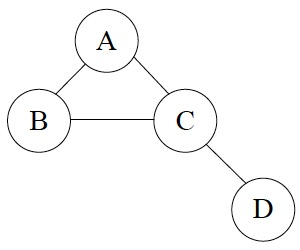
\includegraphics[scale=0.35]{Lab08-figure2.jpg}
 \caption{A undirected graph.}
\end{figure}

\begin{solution}
Since the graph is connected, we can use an improved DFS. First, I will redefine the EXPLORE recurrent function, and then use it in the path search. Note that I use $AddTrace(edge(*))$ to add one component to the path. For example, $AddTrace(edge(v,u))$ stands for add a trace '$v \rightarrow u$' to the path.

For the EXPLORE function:

\begin{minipage}[t]{0.9\textwidth}
\begin{algorithm}[H]
	\BlankLine
	\SetKwInOut{Input}{input}
	\SetKwInOut{Output}{output}
	\caption{EXPLORE}\label{Alg_EXPLORE}
	\Input{A directed graph G=(V,E); a vertex $v \in V$}
	\Output{Find the path which traverses each edge exactly once in each direction}
	\BlankLine
	\If{$v.predecessor$}{$AddTrace(edge(v.predecessor,v))$\;}
	$v.visit \leftarrow True$\;
	\ForEach{$edge(v,u) \in E$}{
	\If{\textbf{not} $u.visit$}{
	$u.predecessor \leftarrow v$\;
	$EXPLORE(u)$\;
	}
	\Else{
	\If{$edge(v,u) \notin Trace$}{/*The edge between v and u had not been went through*/
	$AddTrace(edge(v,u))$\;
	$AddTrace(edge(u,v))$\;
	}
	}
	\If{$v.predecessor$}{$AddTrace(edge(v,v.predecessor))$\;}
	}
\end{algorithm}
\end{minipage}

This is the whole pseudo code:

\begin{minipage}[t]{0.9\textwidth}
\begin{algorithm}[H]
	\BlankLine
	\SetKwInOut{Input}{input}
	\SetKwInOut{Output}{output}
	\caption{GraphSearch}\label{Alg_GraphSearch}
	\Input{A directed graph G=(V,E)}
	\Output{Find the path which traverses each edge exactly once in each direction}
	\BlankLine
	\ForEach{$u \in V$}{
	$u.predecessor\leftarrow None$\;
	$u.visit\leftarrow None$\;
	}
	Randomly choose a vertex $v$\;
	$u.visit\leftarrow True$\;
	$EXPLORE(G,v)$\;
\end{algorithm}
\end{minipage}
\end{solution}

\end{enumerate}

%========================================================================
\end{document}

